\documentclass{article}
\usepackage{etoolbox}
\usepackage{graphicx}

\ifdef{\myoutput}{}{\def\myoutput{concept}}
\ifdef{\myversion}{}{\def\myversion{1}}

\usepackage[output=\myoutput
,numberofversions=4
,version=\myversion
,seed=4
,randomizequestions=true
,randomizeanswers=true
,writeRfile=true
]{mcexam}

\usepackage[margin=0.95in]{geometry}
\usepackage{multicol}

\usepackage{fancyhdr,lastpage}
\pagestyle{fancy}
\fancyhf{}
\renewcommand{\headrulewidth}{1pt} 
\renewcommand{\footrulewidth}{1pt}
\lfoot{\mctheversion}
\rfoot{Page \thepage\ of \pageref{LastPage}}
\lhead{Quiz 3.3 Version \fbox{\myversion} \\ MAT 2000: Introduction to Statistics}
\rhead{Name Print): \hspace{2.5 in}}

\usepackage{calc}
\renewenvironment{setmcquestion}
{\begin{minipage}[t]{\linewidth-\labelwidth}}
	{\end{minipage}\par}
	
\renewenvironment{setmcquestioninstruction}
{\begin{minipage}{\textwidth}}
	{\end{minipage}}
	
\renewenvironment{setmcanswers}{}{}
\setlist[setmcquestions]{label=\mcquestionlabelfmt{*}.
	,ref=\mcquestionlabelfmt{*}
	,itemsep=0.5\baselineskip
	,topsep=1\baselineskip
}

\renewcommand\mcversionlabelfmt[1]{\arabic{#1}}

%\mcifoutput{exam}{
%	\AtEndDocument{\ifodd\value{page}
%		\newpage\thispagestyle{empty}\hbox{This page intentionally left blank.}\newpage\thispagestyle{empty}\hbox{}
%		\else
%		\newpage\thispagestyle{empty}\hbox{}
%		\fi}
%}

\raggedbottom

\begin{document}
	Circle the correct answer for each question.  If you're unsure, you can write numbers 1, 2, 3, etc. next to the choices to get partial credit.\\[.5cm]
	\begin{mcquestions}
		\question Most experts recommend college students get at least 8 hours of sleep per night. A random sample is collected of 112 students at a college by asking how many hours of sleep each student got last night. The sample mean amount of sleep last night was 7.6 hours, with a sample standard deviation of 2.1 hours. The sample distribution of hours of sleep was slightly skewed right.
		
		Use the sample results to estimate the standard error of the sampling distribution of sample means.
		\begin{mcanswerslist}
			\answer 2.1
			\answer[correct] 0.198
			\answer 7.6
			\answer 0.718			
		\end{mcanswerslist}
		
		\begin{mcquestioninstruction}
			Adult male polar bears are expected to weigh, on average, 370 kg, but there is concern by some scientists that because of recent warmer winters that polar bears might be struggling to gain weight. The US Geological Survey (USGS) conducted a study in the Southern Beaufort Sea on the weight of polar bears. Eighty-three adult male polar bears were captured between March and May of the years 1990 and 2006 and their weights were recorded. The sample mean weight was 324.6 kg, and the sample standard deviation was 88.3 kg.
			
			A histogram of the 83 polar bear weights in the sample is shown below.
			\begin{center}
				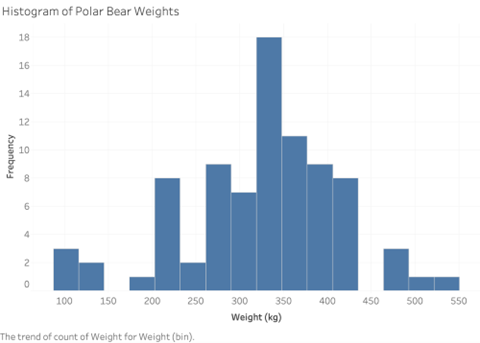
\includegraphics{polar_bears.png}
			\end{center}
		\end{mcquestioninstruction}
	
		\question Are the validity conditions for theory-based inference met for these data?
		\begin{mcanswerslist}
			\answer Yes, since at least 10 polar bears weighed more than 370 kg and at least 10 weighed less than 370 kg.
			\answer[correct] Yes, since the sample size is larger than 20 and the sample distribution is not strongly skewed.
			\answer No, since the sample distribution is slightly skewed left.
			\answer Unable to determine.
		\end{mcanswerslist}
		
		\question[follow] What are the appropriate null and alternative hypotheses?
		\begin{mcanswerslist}
			\answer $H_0:\overline x = 370$ versus $H_A:\overline x \neq 370$
			\answer  $H_0:\overline x = 370$ versus $H_A:\overline x < 370$
			\answer[correct]  $H_0:\mu = 370$ versus $H_A:\mu \neq 370$
			\answer  $H_0:\mu = 370$ versus $H_A:\mu < 370$		
		\end{mcanswerslist}
		
		\question[follow] The sample mean of 324.6 kg lies \_\_\_(1)\_\_\_\_ standard errors \_\_\_(2)\_\_\_ the expected average polar bear weight of 370 kg.
		\begin{mcanswerslist}
			\answer 4.68, above
			\answer[correct] 4.68, below
			\answer 0.51, above
			\answer 0.51, below
		\end{mcanswerslist}
		
		\question[follow] A theory-based inference applet gives a p-value less than 0.00001. Do these results provide evidence that the true mean weight of polar bears is less than 370 kg?
		\begin{mcanswerslist}
			\answer No, since the sample results could have happened by chance.
			\answer Yes, since 324.6 kg is less than 370 kg.
			\answer[correct] Yes, since the p-value is small.
			\answer No, since the p-value is large.
		\end{mcanswerslist}
		
		\question If the p-value is very small, which of the following is true?
		\begin{mcanswerslist}
			\answer[correct] Very strong evidence exists against the null hypothesis.
			\answer Very strong evidence exists against the alternative hypothesis.
			\answer The null hypothesis has been proven.
			\answer The alternative hypothesis has been proven.
		\end{mcanswerslist}
		
	\end{mcquestions}
\end{document}